\documentclass[tikz,border=6pt]{standalone}
\usepackage[T1]{fontenc}
\usepackage[utf8]{inputenc}
\usepackage{pgfplots}
\usepgfplotslibrary{groupplots}
\usetikzlibrary{calc}
\pgfplotsset{compat=1.18}
\begin{document}
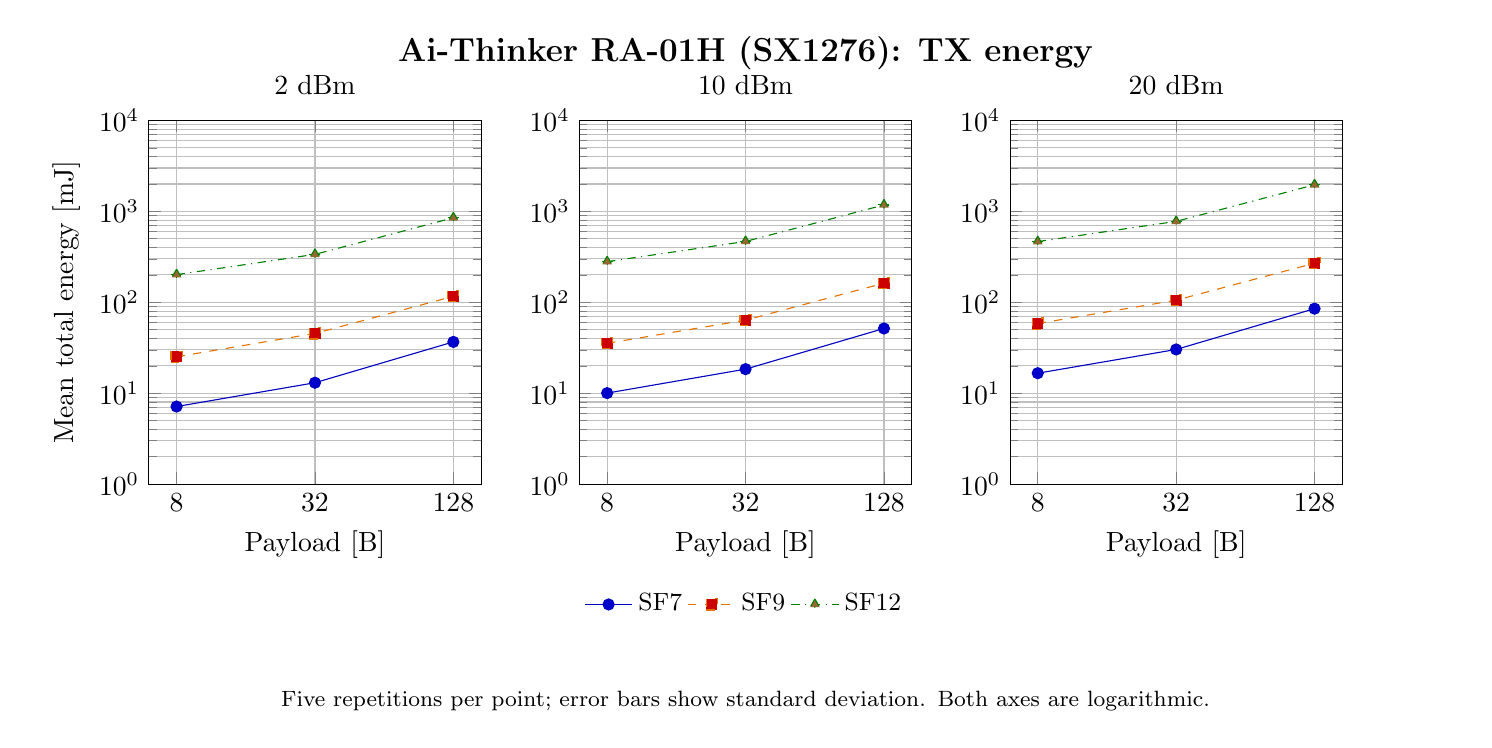
\begin{tikzpicture}
\begin{groupplot}[/pgf/number format/use comma, group style={group size=3 by 1, horizontal sep=1.25cm},
  width=5.8cm,height=6.2cm,xmode=log,log basis x=2,ymode=log,log basis y=10,ymin=1,ymax=10000,
  xtick={8,32,128},xticklabels={8,32,128},grid=both,xlabel={Payload [B]},
  legend style={draw=none,fill=none,font=\small,at={(0.5,-0.27)},anchor=north,legend columns=-1}]
% TX energy
\nextgroupplot[title={2 dBm},ylabel={Mean total energy [mJ]}]
\addplot+[blue!75!black,solid,mark=*,error bars/.cd,y dir=both,y explicit] coordinates {(8,7.12674686) +- (0,0.00420563582) (32,13.0236351) +- (0,0.00558522052) (128,36.6359436) +- (0,0.022582668)};
\addplot+[orange!90!black,dashed,mark=square*,error bars/.cd,y dir=both,y explicit] coordinates {(8,25.1270279) +- (0,0.0138518963) (32,45.3811967) +- (0,0.0205030224) (128,116.24027) +- (0,0.0425829567)};
\addplot+[green!50!black,dashdotted,mark=triangle*,error bars/.cd,y dir=both,y explicit] coordinates {(8,201.225922) +- (0,0.0413228502) (32,336.269998) +- (0,0.133471406) (128,849.493001) +- (0,0.136370844)};
\nextgroupplot[title={10 dBm}]
\addplot+[blue!75!black,solid,mark=*,error bars/.cd,y dir=both,y explicit] coordinates {(8,10.0157557) +- (0,0.0570689228) (32,18.3759594) +- (0,0.072756413) (128,51.4686764) +- (0,0.235137108)};
\addlegendentry{SF7}
\addplot+[orange!90!black,dashed,mark=square*,error bars/.cd,y dir=both,y explicit] coordinates {(8,35.3335188) +- (0,0.154363465) (32,63.5958279) +- (0,0.247917848) (128,162.072167) +- (0,0.794289049)};
\addlegendentry{SF9}
\addplot+[green!50!black,dashdotted,mark=triangle*,error bars/.cd,y dir=both,y explicit] coordinates {(8,279.701915) +- (0,0.667315813) (32,466.470584) +- (0,1.15765999) (128,1175.48268) +- (0,2.24498054)};
\addlegendentry{SF12}
\nextgroupplot[title={20 dBm}]
\addplot+[blue!75!black,solid,mark=*,error bars/.cd,y dir=both,y explicit] coordinates {(8,16.5724889) +- (0,0.0414483964) (32,30.2445219) +- (0,0.0429773056) (128,85.0036059) +- (0,0.236442018)};
\addplot+[orange!90!black,dashed,mark=square*,error bars/.cd,y dir=both,y explicit] coordinates {(8,58.3411324) +- (0,0.137141565) (32,105.308109) +- (0,0.310246775) (128,268.829675) +- (0,0.863137163)};
\addplot+[green!50!black,dashdotted,mark=triangle*,error bars/.cd,y dir=both,y explicit] coordinates {(8,464.664055) +- (0,0.639051593) (32,775.881614) +- (0,0.444753553) (128,1958.53726) +- (0,0.898306677)};
\end{groupplot}
\node[font=\bfseries\large] at ($(group c2r1.north)+(0,0.85cm)$) {Ai-Thinker RA-01H (SX1276): TX energy};
\node[font=\footnotesize,align=center,text width=18cm] at ($(group c2r1.south)+(0,-2.75cm)$) {Five repetitions per point; error bars show standard deviation. Both axes are logarithmic.};
\end{tikzpicture}
\end{document}
